
In order to evaluate the proposed approach of axiom weakening, specifically for its application in the context of automatic repair of ontologies, we need a way to compare the quality of different possible repairs. As has already been discussed in \cite{troquard2018repairing}, the problem of deciding which of two possible repaired ontologies $\Omc_1$ or $\Omc_2$ is preferable is not generally well-defined. As such, this thesis will use the same measure defined for the experimental evaluation in \cite{troquard2018repairing}. The main idea is to use the size of the \emph{inferred class hierarchy} to evaluate the amount of ``information'' a repair is able to retain.

\begin{definition}
  The \emph{inferred class hierarchy} of an ontology $\Omc$ is given by
  \begin{align*}
    \Inf(\Omc) = \{ A \sqsubseteq B \mid A, B \in N_C \text{ and } \Omc \models A \sqsubseteq B \} \enspace.
  \end{align*}
\end{definition}

To compare the relative amount of information between two ontologies, we compare them based on their differences in the inferred class hierarchy. We use for this purpose the \emph{inferred information content} (IIC) as defined in \cite{troquard2018repairing}.

\begin{definition}
  The \emph{inferable information content} of an ontology $\Omc_1$ with respect to another ontology $\Omc_2$ is given by
  \begin{align*}
    \qual(\Omc_1, \Omc_2) = \frac{| \Inf(\Omc_1) \setminus \Inf(\Omc_2) |}{|\Inf(\Omc_1) \setminus \Inf(\Omc_2)| + |\Inf(\Omc_2) \setminus \Inf(\Omc_1)|} \enspace,
  \end{align*}
  where $|X|$ is the cardinality of the set $X$.
\end{definition}

The IIC of an ontology $\Omc_1$ with respect to a second ontology $\Omc_2$, written $\qual(\Omc_1, \Omc_2)$, is a number between $0$ and $1$. Value closer to $0$ indicates that $\Omc_1$ contains more ``information'' than $\Omc_2$, while a value towards $1$ indicates the opposite. Inferred hierarchy axioms common to both ontologies do not influence the results, and if $\Omc_2$ is entailed by $\Omc_1$, then the IIC of $\Omc_1$ with respect to $\Omc_2$ is always $1$. If both $\Omc_1$ and $\Omc_2$ have some inferences that are not shared by the other ontology, the IIC will be strictly between $0$ and $1$. Note that if the cardinality of the inferred class hierarchy is larger for one ontology, then it will also be the one preferred by the IIC. Some weaknesses of this measure when it comes to evaluating repairs, like the fact that only atomic concepts are considered, have already been discussed in \cite{troquard2018repairing}. For the case of repairing \SROIQ ontologies this is even more relevant, since the role hierarchy is entirely ignored.

The evaluation starts by first making the ontologies inconsistent. This has been achieved by repeatedly adding axioms to the ontology until it was no longer consistent. The newly added axioms were generated by strengthening randomly selected axioms of the ontology. Axioms are strengthened by applying an axiom strengthening operator, that is equivalent to the axiom weakening operator in \cref{def:weaken}, except for swapping the generalization and specialization operators and not removing axiom by using $\bot \sqsubseteq \top$. An axiom $\alpha'$ is stronger than another axiom $\alpha$ with respect to the ontology $\Omc$ if $\alpha' \models_\Omc \alpha$. Note that this is only a useful characterization if $\alpha \not\in \Omc$. It was ensured that the added axioms on their own were not inconsistent. After making the ontology inconsistent, it was repaired using different automatic repair algorithms. Each inconsistent ontology was repaired once with the repair algorithm using the axiom weakening operator presented in \cref{algo:repair-weaken} and once using \cref{algo:repair-remove}. As can be seen in \cref{ex:alc-weakening}, choosing a maximal consistent subset can sometimes lead to less information loss that using the weakening based algorithm. To experimentally evaluate how good weakening performs against maximal consistent subset base repair on average, the repair was also performed by selecting a randomly sampled maximal consistent subset.

\begin{algorithm}[ht]
  \begin{algorithmic}
    \While{$\Omc$ is inconsistent}
    \State $\phi_\textnormal{bad} \gets \textsc{FindBadAxiom}(\Omc)$
    \State $\Omc \gets \Omc \setminus \{\phi_\textnormal{bad}\}$
    \EndWhile
    \State Return $\Omc$
  \end{algorithmic}
  \caption{\textsc{RepairOntologyRemove}($\Omc$)}
  \label{algo:repair-remove}
\end{algorithm}

This process, both making the ontology inconsistent and repairing it, was repeated one hundred times for each ontology, and the IIC was computed between the results of the different repair methods. The evaluation was performed using a randomly sampled maximal consistent subset as the reference ontology and by randomly sampling $16$ minimal inconsistent subsets during the selection of bad axioms in \textsc{FindBadAxiom}(\Omc). To obtain comparable results, both \textsc{RepairOntologyRemove}($\Omc$) and \textsc{RepairOntologyWeakening}($\Omc$) use the same implementation of \textsc{FindBadAxiom}($\Omc$). While the utilized OWL 2 DL reasoners are all highly optimized, they exhibit undesirable performance in some edge cases. Mostly they are fast to perform reasoning task like checking for consistency or entailment in the selected ontologies. However, when performance pitfalls are encountered, they may require significantly more time, making the computation required for repair unreasonably slow. For this reason a timeout of 5 minutes was placed on the repairs execution and the outputs of runs that did not complete within this time limit where discarded and replaced by new runs. The results of these experiments are listed in \cref{table:results} and shown in \cref{fig:results-remove} and \cref{fig:results-mcs}.

\begin{table}[ht]
  \scriptsize
  \centering
  \begin{tabular}{|l|cc|}
    \hline
    & IIC w.r.t. repair by removal & IIC w.r.t. maximal consistent subset \\
    \hline
    admin & 0.53 [0.47; 0.59] & 0.39 [0.31; 0.47] \\
    ahso & 0.56 [0.50; 0.62] & 0.51 [0.44; 0.57] \\
    cdao & 0.53 [0.44; 0.61] & 0.53 [0.45; 0.61] \\
    cdpeo & 0.50 [0.45; 0.55] & 0.22 [0.16; 0.28] \\
    covid19-ibo & 0.70 [0.65; 0.75] & 0.63 [0.57; 0.69] \\
    ecp & 0.74 [0.67; 0.81] & 0.36 [0.28; 0.44] \\
    emo & 0.69 [0.63; 0.75] & 0.60 [0.53; 0.66] \\
    evi & 0.49 [0.43; 0.55] & 0.59 [0.53; 0.66] \\
    falls & 0.78 [0.71; 0.85] & 0.49 [0.41; 0.58] \\
    fo & 0.50 [0.44; 0.57] & 0.70 [0.62; 0.76] \\
    gbm & 0.59 [0.52; 0.66] & 0.52 [0.44; 0.59] \\
    gfvo & 0.56 [0.49; 0.62] & 0.54 [0.49; 0.60] \\
    koro & 0.51 [0.45; 0.57] & 0.37 [0.29; 0.45] \\
    lico & 0.55 [0.48; 0.62] & 0.53 [0.46; 0.60] \\
    mamo & 0.52 [0.44; 0.60] & 0.68 [0.61; 0.74] \\
    mpio & 0.70 [0.63; 0.76] & 0.73 [0.67; 0.78] \\
    pizza & 0.56 [0.49; 0.64] & 0.61 [0.53; 0.68] \\
    provo & 0.50 [0.43; 0.56] & 0.55 [0.49; 0.62] \\
    qudt & 0.96 [0.93; 0.99] & 0.44 [0.35; 0.55] \\
    trans & 0.58 [0.52; 0.64] & 0.43 [0.35; 0.52] \\
    triage & 0.53 [0.46; 0.60] & 0.53 [0.46; 0.60] \\
    vio & 0.46 [0.37; 0.55] & 0.49 [0.40; 0.57] \\
    \hline
    Overall & 0.59 [0.57; 0.61] & 0.52 [0.50; 0.54] \\
    \hline
  \end{tabular}
  \caption{Results of the evaluation. IIC is given as mean and 95\% confidence interval in brackets.}
  \label{table:results}
\end{table}

\begin{figure}[ht]
  \centering
  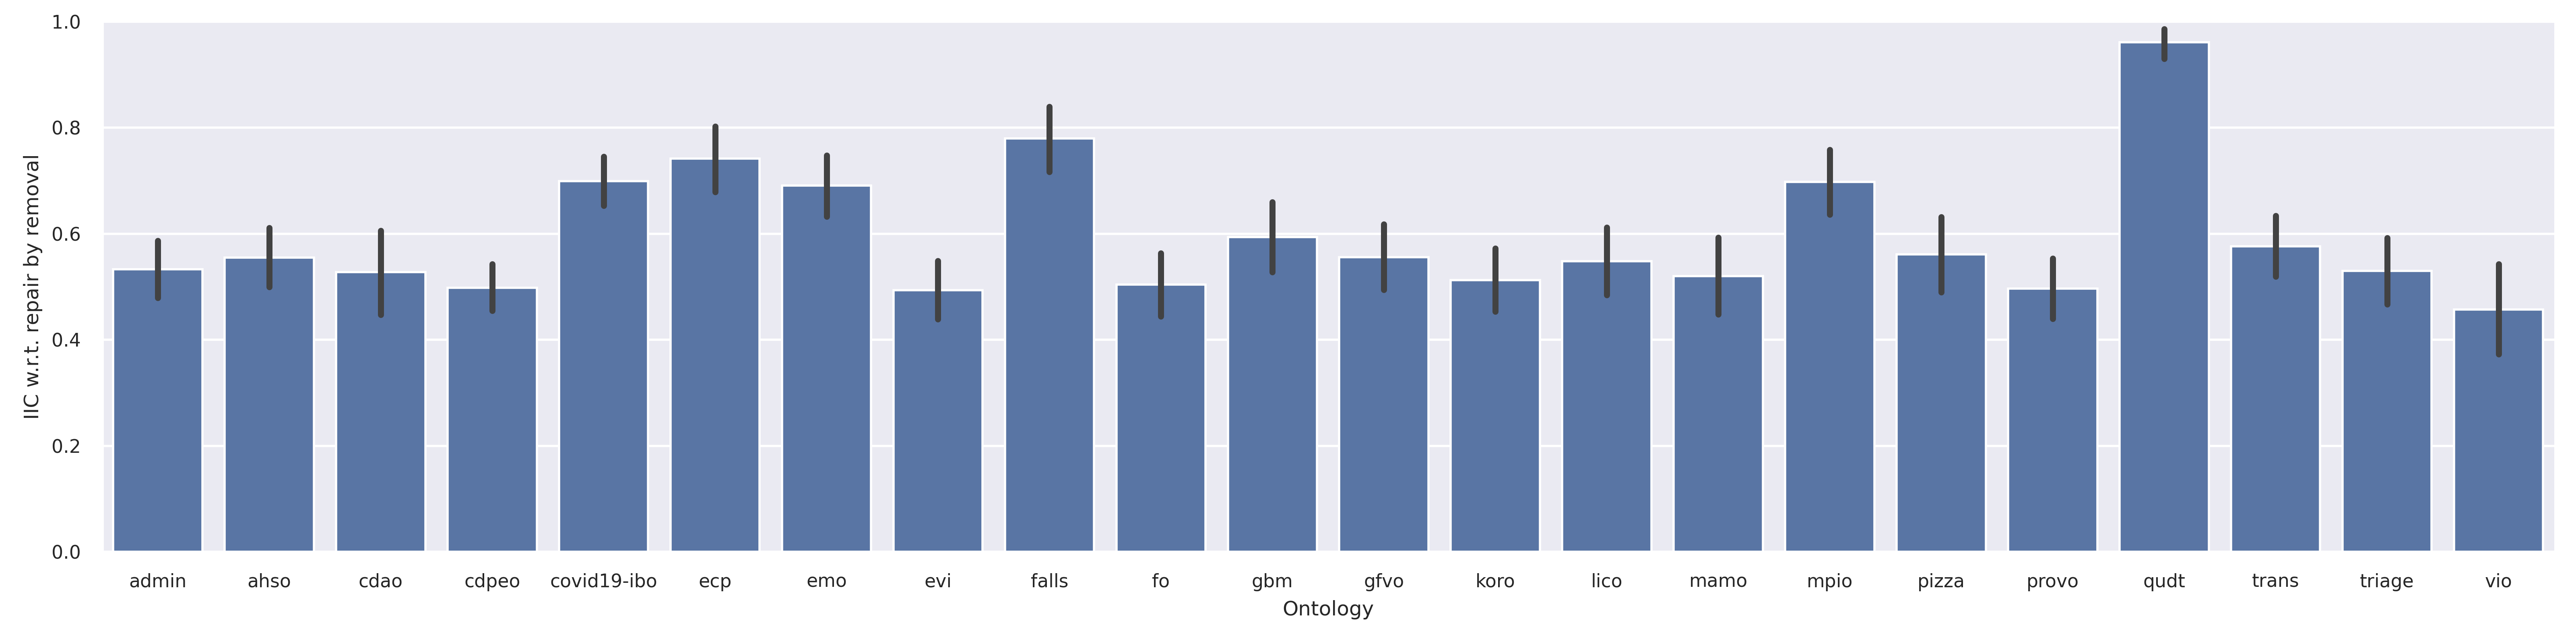
\includegraphics[width=\textwidth]{resources/iic-remove-ontology-bar.png}
  \caption{Mean IIC with respect to repair via removal per ontology. The error bars show the 95\% confidence interval.}
  \label{fig:results-remove}
\end{figure}

\begin{figure}[ht]
  \centering
  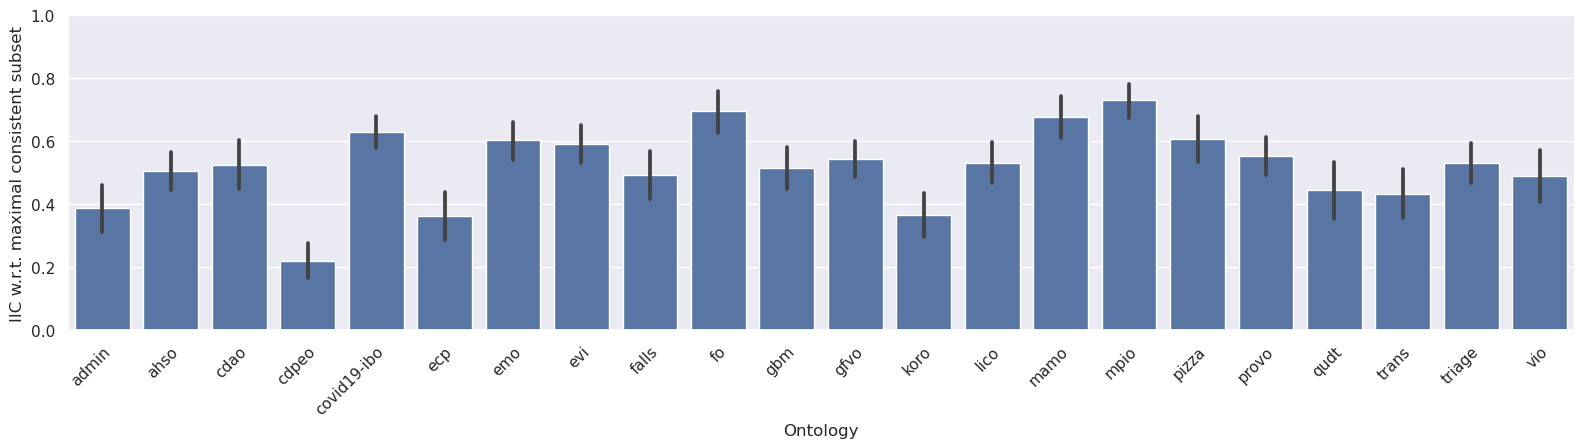
\includegraphics[width=\textwidth]{resources/iic-mcs-ontology-bar.png}
  \caption{Mean IIC with respect to a random maximal consistent subset per ontology. The error bars show the 95\% confidence interval.}
  \label{fig:results-mcs}
\end{figure}

The results of the evaluation suggest that the repair by weakening is on average about as good or better than the repair by removal of axioms. While this supports the conclusion in \cite{troquard2018repairing} that weakening is able to retain more information than removal, the observed advantage was worse than what has been observed in \cite{troquard2018repairing}.

In contrast, it can be seen that the repair using weakening is not in general better than choosing a random maximal consistent subset. There are ontologies for which the repairs by weakening are on average significantly worse when comparing using IIC. This is, however, a somewhat unequal comparison. We have seen in \cref{ex:alc-weakening} also a situation in which weakening performs worse when it comes to preserving information compared to choosing a maximally consistent subset. An alternative repair algorithm could start with a maximal consistent subset and use weakening to add in more information from the remaining axioms. Still, this result suggests that the heuristic used for selecting bad axioms is not reliable for preserving information, at least with respect to the chosen measure. Also, it has not been closely studied what causes the repair by weakening to significantly lose for some ontologies, while being clearly preferred in others. Interestingly there are also some cases in which the weakening based repair performs better against a random maximal consistent subset than against the repair by removal.
